% !TEX root = ../STP_journal.tex
\subsubsection{Least Restrictive Control}
Fig. \ref{fig:lrc_traj} shows the simulated trajectories in the situation where each vehicle assumes that higher-priority vehicles use the least restrictive control to reach their targets, as described in \ref{sec:lrc}. Fig. \ref{fig:lrc_rs3} shows the BRS and induced obstacles for $\veh_3$.

$\veh_1$ (red) takes a relatively straight path to its target. From the perspective of other vehicles, large obstacles are induced by $\veh_1$, since lower-priority vehicles make the weak assumption that higher-priority vehicles are using the least restrictive control. Because the induced obstacles are so large, it is faster for lower-priority vehicles to wait until higher-priority vehicles pass by than to move around higher-priority vehicles. As a result, vehicles never form a dense configuration, and their trajectories are relatively straight, indicating that vehicles take a short path to the target after higher-priority vehicles pass by. This is also indicated by the early $\ldt_i$ values for the four vehicles, $-1.35, -1.97, -2.66$ and $-3.39$, respectively. Compared to the centralized control method, $\ldt_i$'s are significantly earlier for all vehicles, except $\veh_1$, the highest-priority vehicle, since it need not account for any moving obstacles. 

From $\veh_3$'s (green) perspective, the large obstacles induced by $\veh_1$ and $\veh_2$ are shown in Fig. \ref{fig:lrc_rs3} as the black boundary. As the BRS (green boundary) evolves over time, its growth gets inhibited by the large obstacles for a long time, from $t=-0.89$ to $t=-1.39$. Eventually, the boundary of the BRS reaches the initial state of $\veh_3$ at $t = \ldt_3 = -2.66$.

\begin{figure}
  \centering
  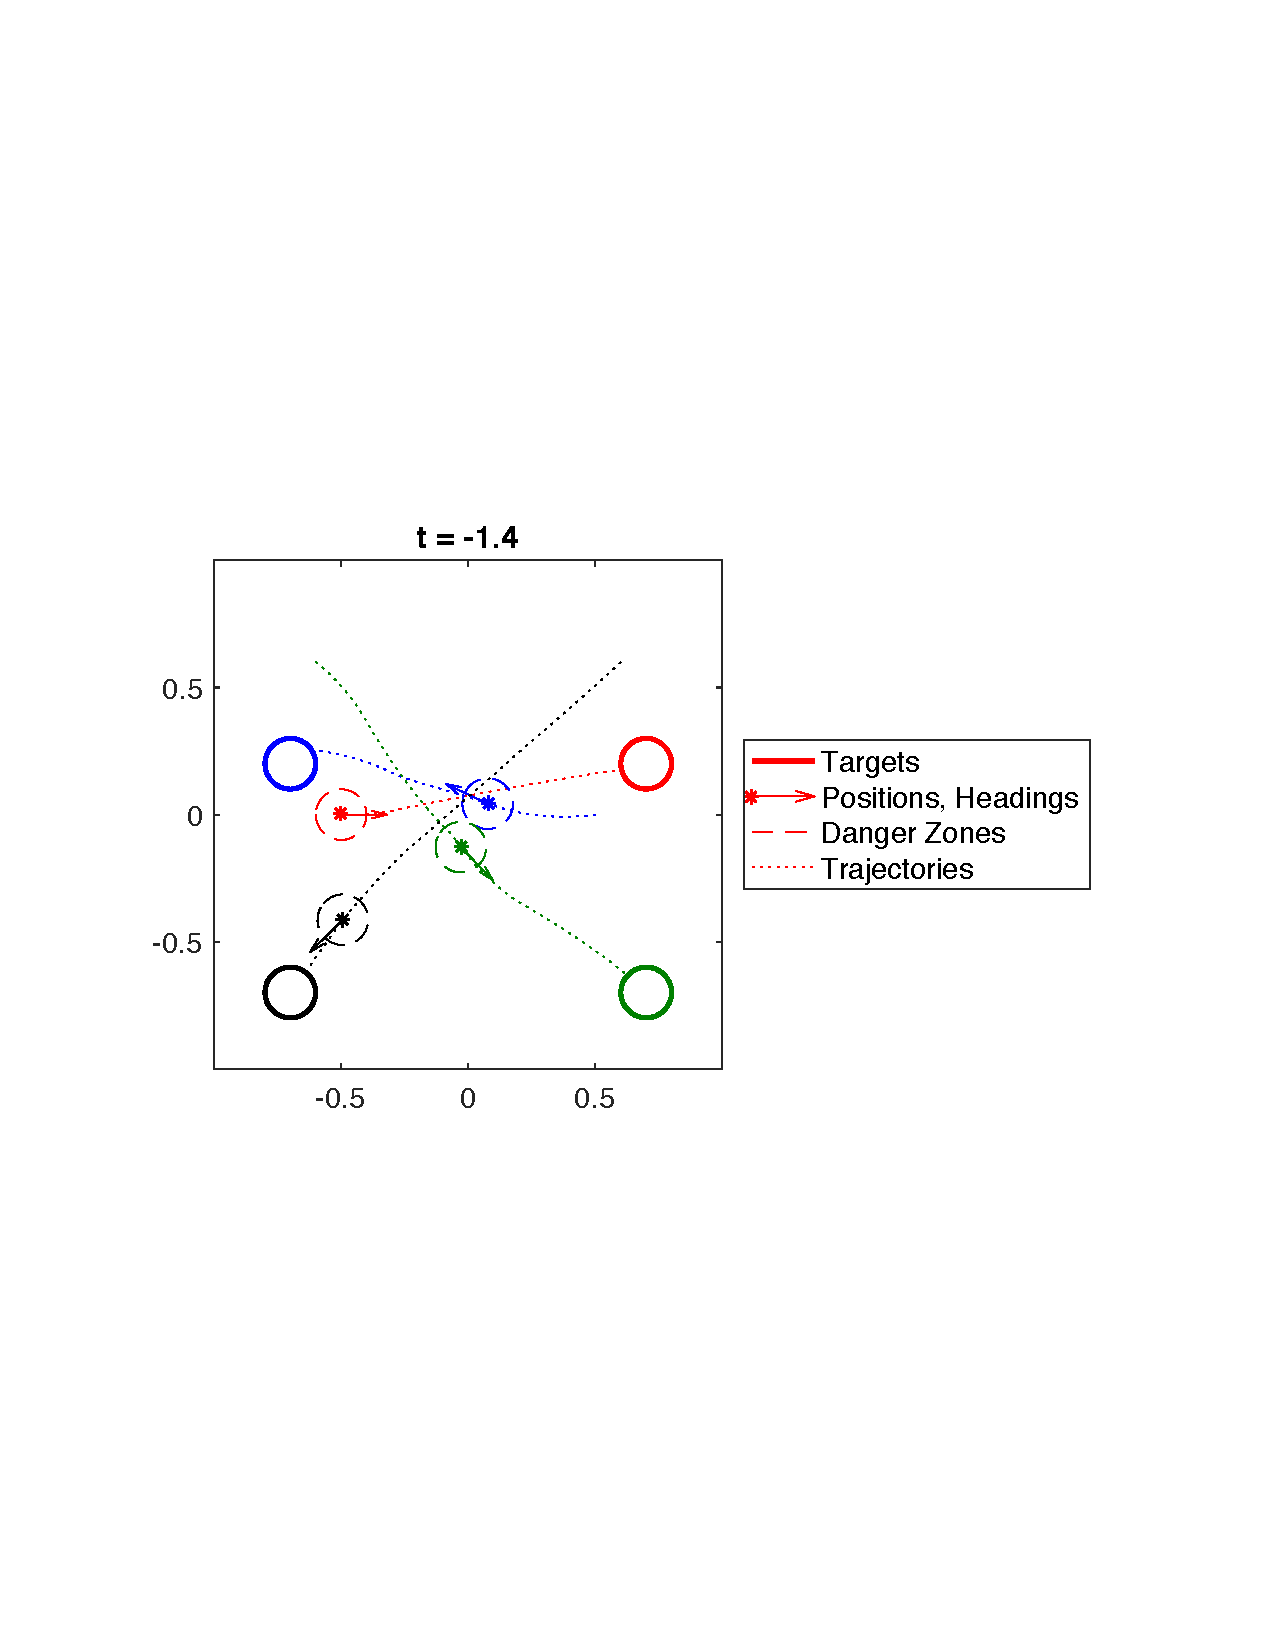
\includegraphics[width=0.8\columnwidth]{fig/lrc_traj}
  \caption{Simulated trajectories in the least restrictive control method. All vehicles start moving before $\veh_1$ starts, because the large obstacles make it optimal to wait until higher priority vehicles pass by, leading to earlier $\ldt_i$'s. }
  \label{fig:lrc_traj}
\end{figure}

\begin{figure}
  \centering
  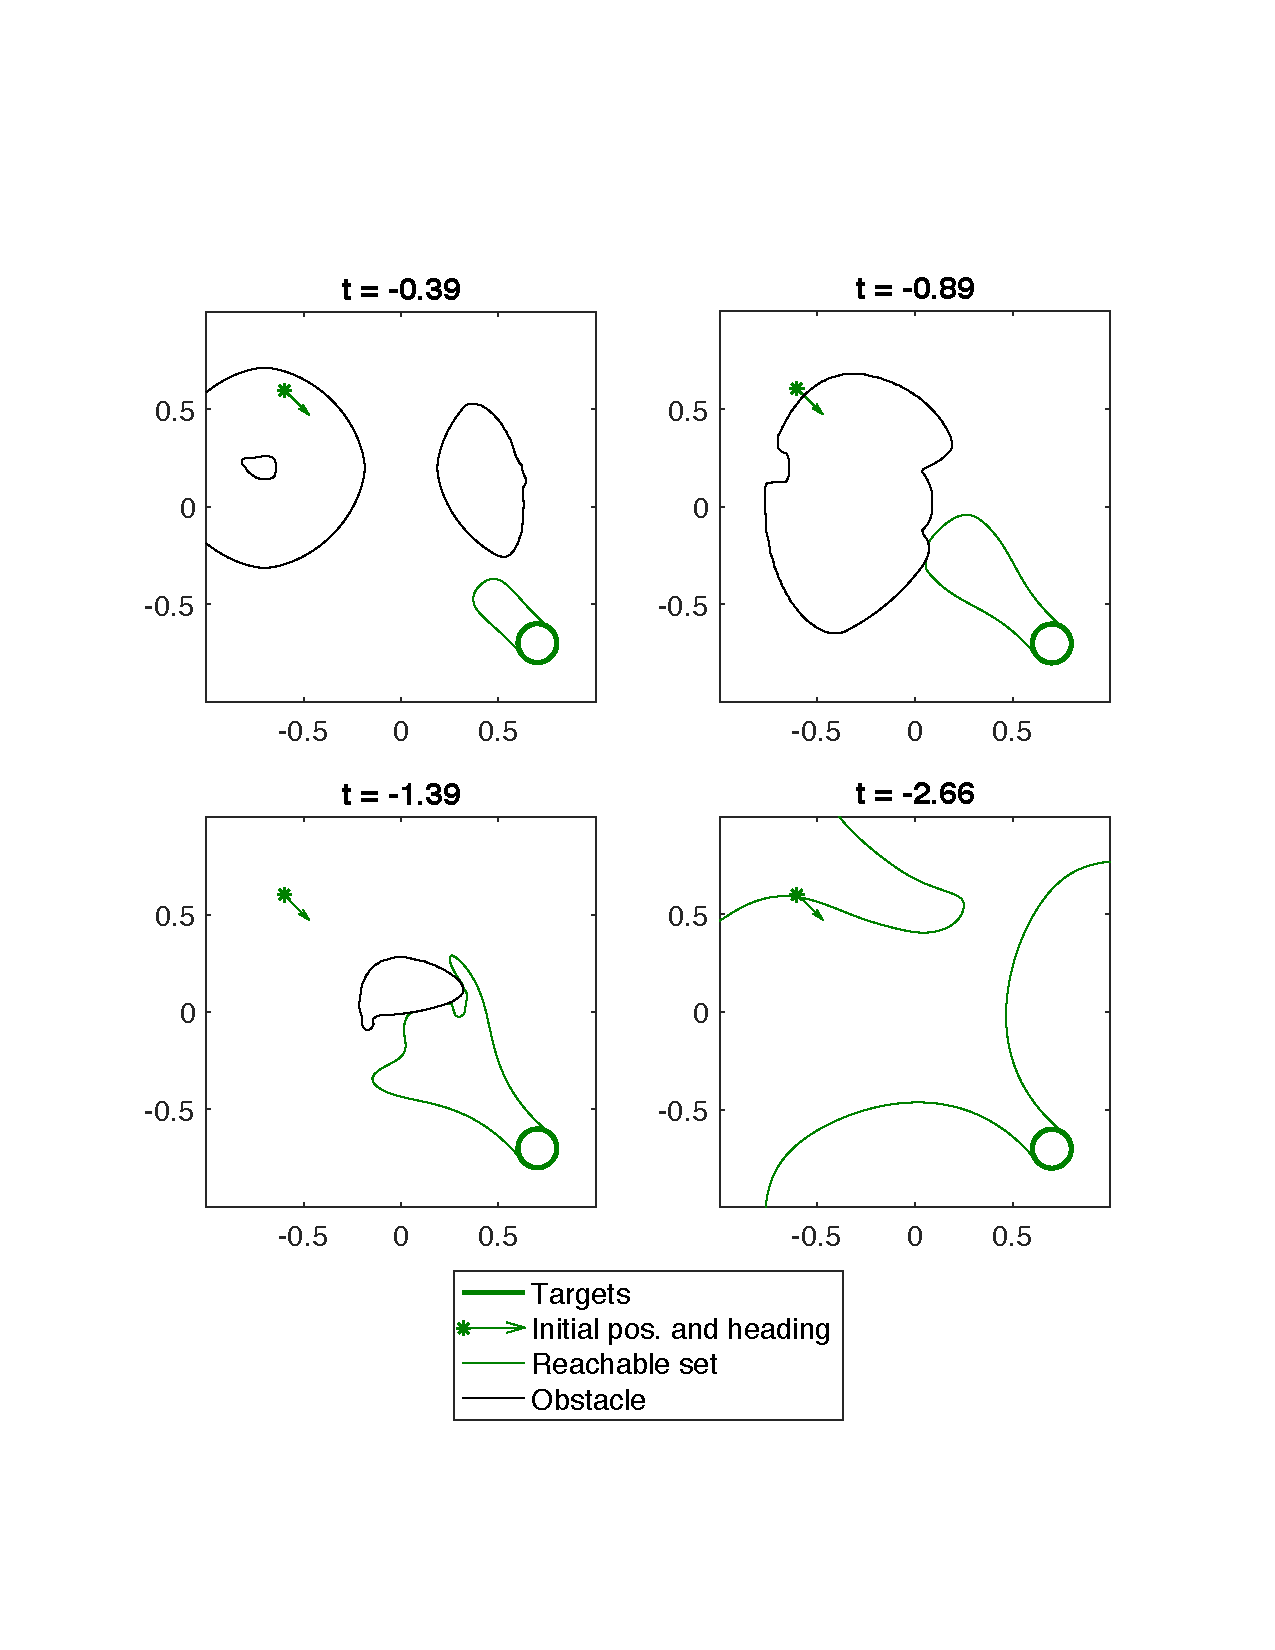
\includegraphics[width=0.9\columnwidth]{fig/lrc_rs3}
  \caption{Evolution of the BRS for $\veh_3$ in the least restrictive control method. In this case, $\ldt_3=-2.66$, significantly earlier than that in the centralized control method ($-1.94$), reflecting the impact of larger induced obstacles.}
  \label{fig:lrc_rs3}
\end{figure}